\section{Attribute-Based Encryption}

Attribute-Based Encryption (ABE) was introduced in 2005 by Sahai and Waters \cite{Sahai}.
It enables an access control mechanism over encrypted data: both users’ private keys and ciphertexts are associated with a set of ascribed attributes or some policy over them.
A user is then able to decrypt a ciphertext if there is a match between his private key and the ciphertext, whereas in traditional PKE schemes messages are encrypted to one particular user only.
\newline\newline
ABE comes in two flavors, namely Ciphertext-Policy (CP) ABE and Key-Policy (KP) ABE.

\paragraph*{CP-ABE}
In Ciphertext-Policy ABE, Alice wants to encrypt a message and can express any access policy, stating what kind of receivers will be able to decrypt the ciphertext.
Such a policy is specified in terms of access structure over receiver attributes.
Each user is indeed given a private key by the authority on the basis of its attributes.
Such a user can decrypt a ciphertext if his attributes satisfy the access policy associated with the ciphertext.
In figure \ref{fig:cp_abe_example} there is an illustration for a CP-ABE example.
\begin{figure}[ht]
    \centering
    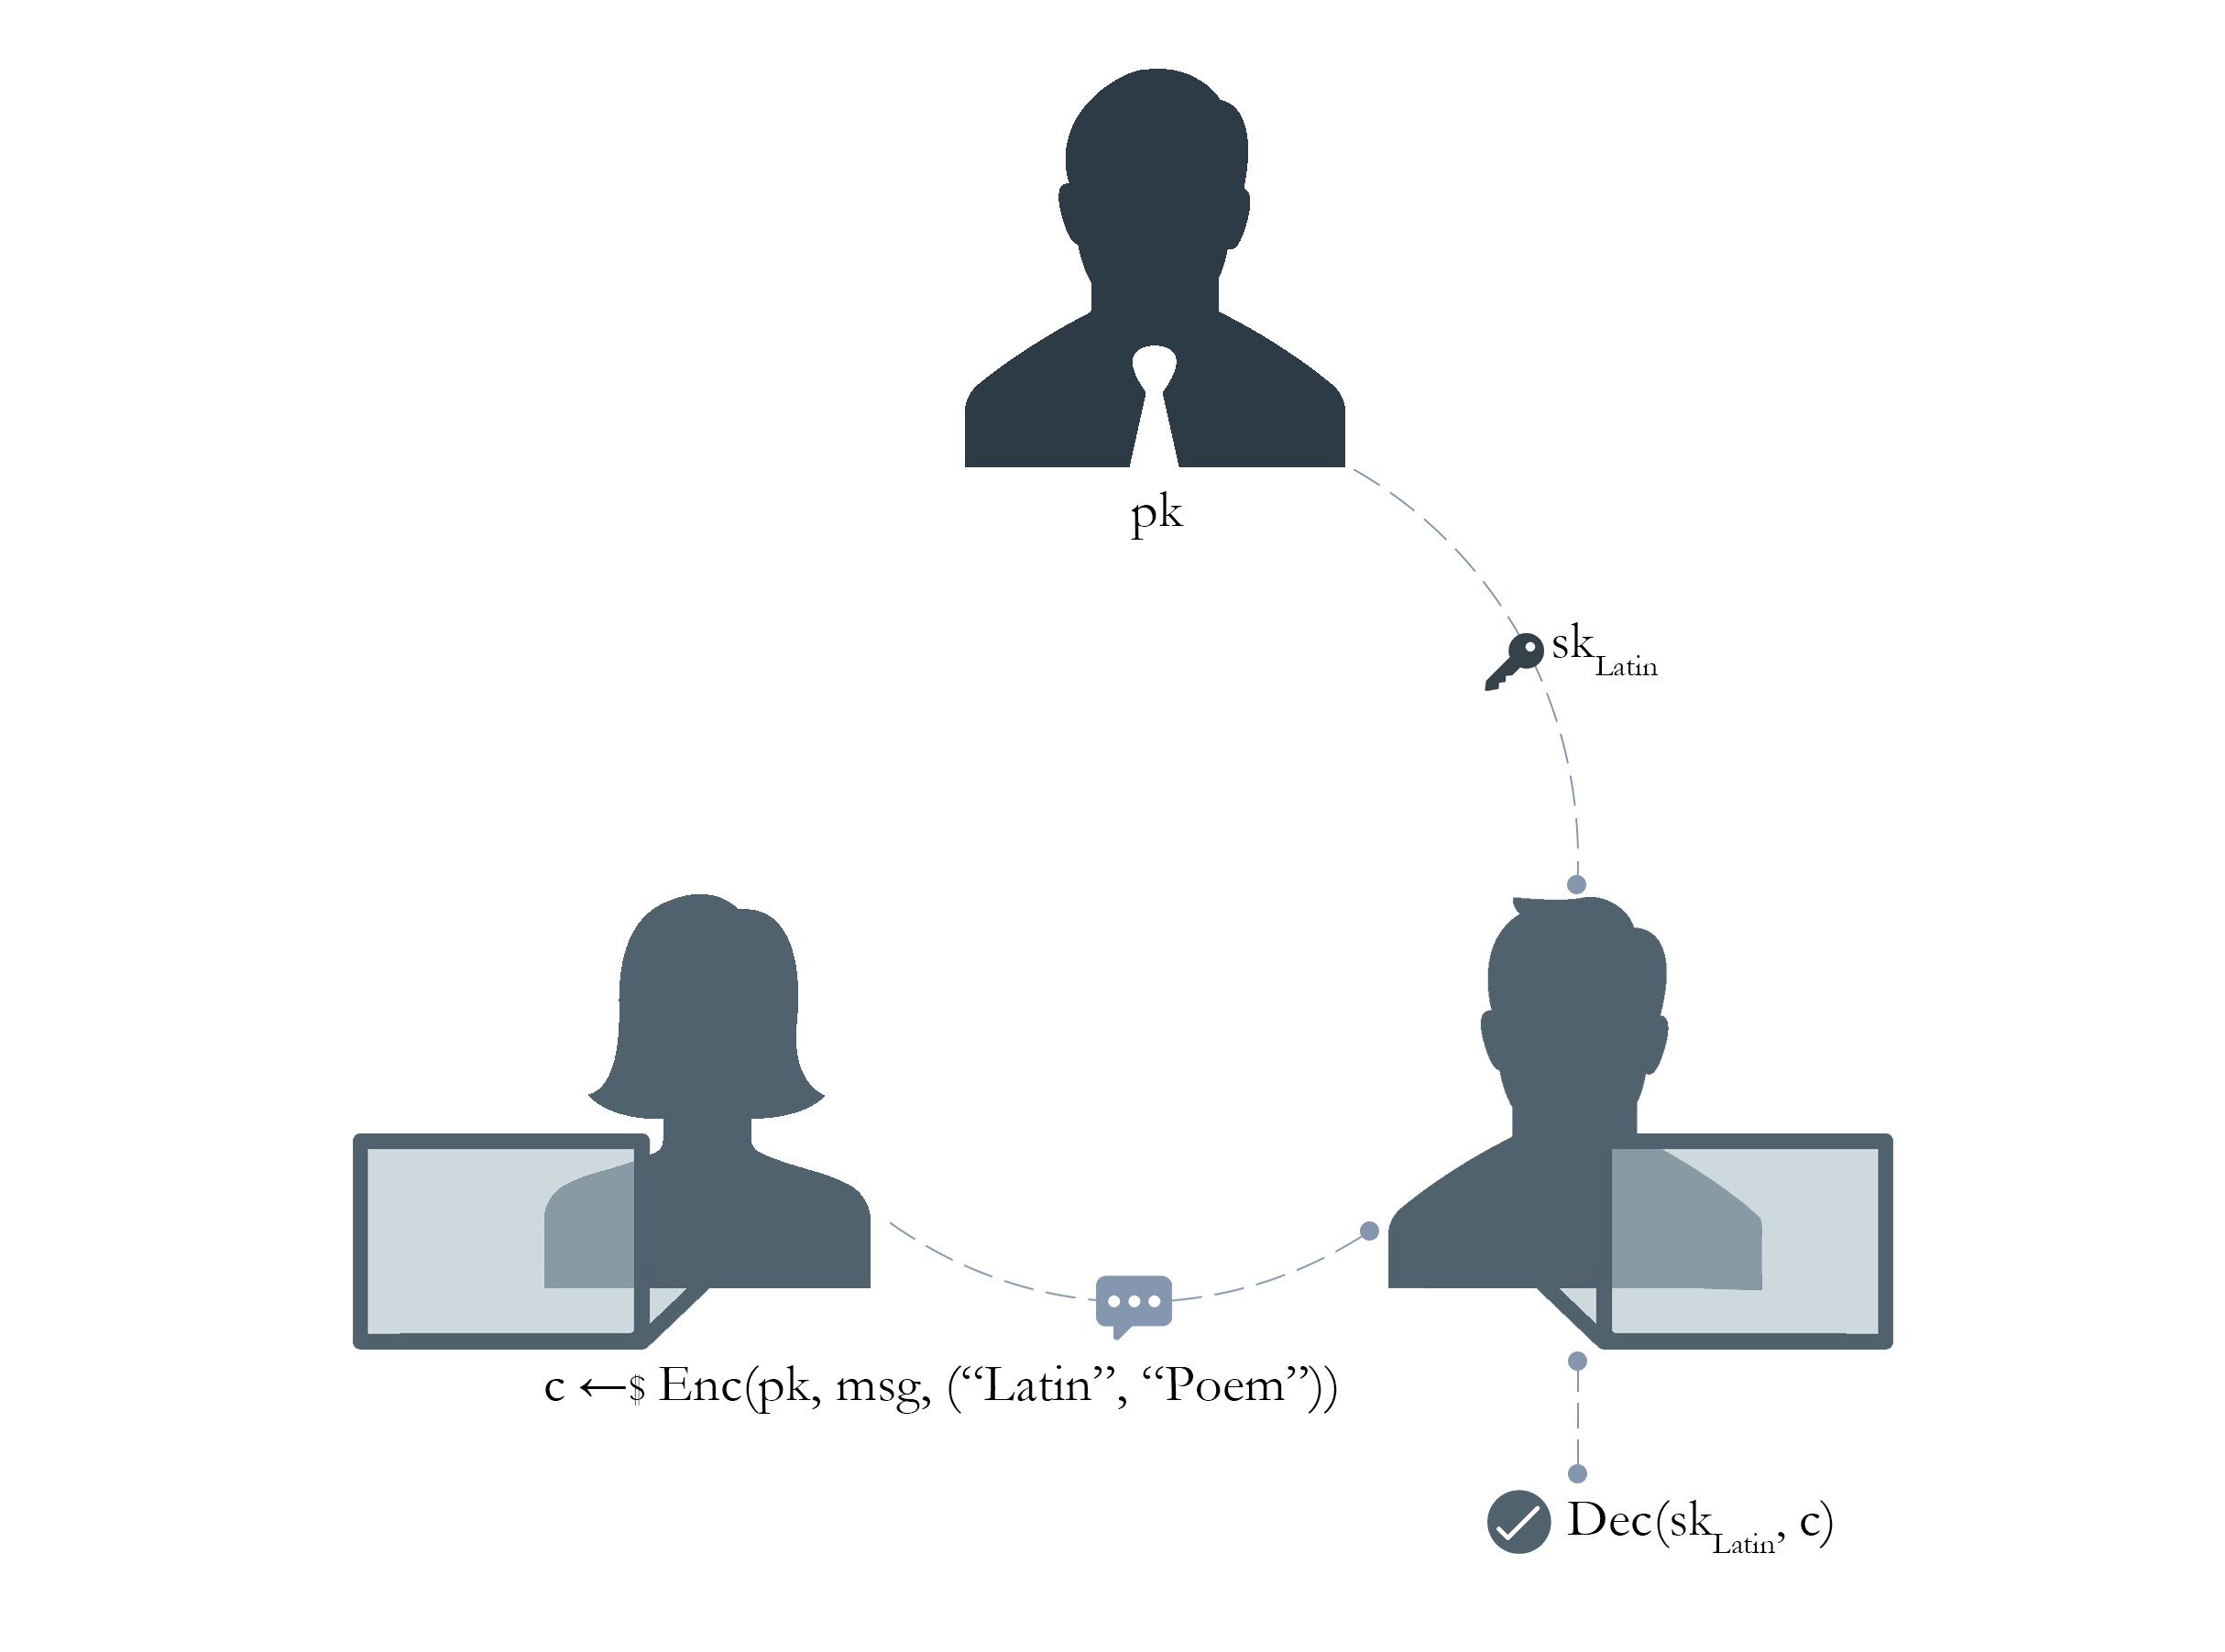
\includegraphics[width=0.8\linewidth]{images/cp_abe.png}
    \caption{CP-ABE example. Alice wants her message to be decrypted by anyone who lives in Italy and was born in 1990. Bob lives in Milan and was born in 1994, so receives a private key associated with his attributes; since there is not a match, he is not able to recover the message.}
    \label{fig:cp_abe_example}
\end{figure}

\paragraph*{KP-ABE}
In Key-Policy ABE, instead, the roles of an attribute set and an access policy are swapped.
Indeed, attribute sets are used to annotate the ciphertexts and access policies over these attributes are associated with users’ secret keys.
In figure \ref{fig:kp_abe_example} there is an illustration for a KP-ABE example.
\begin{figure}[ht]
    \centering
    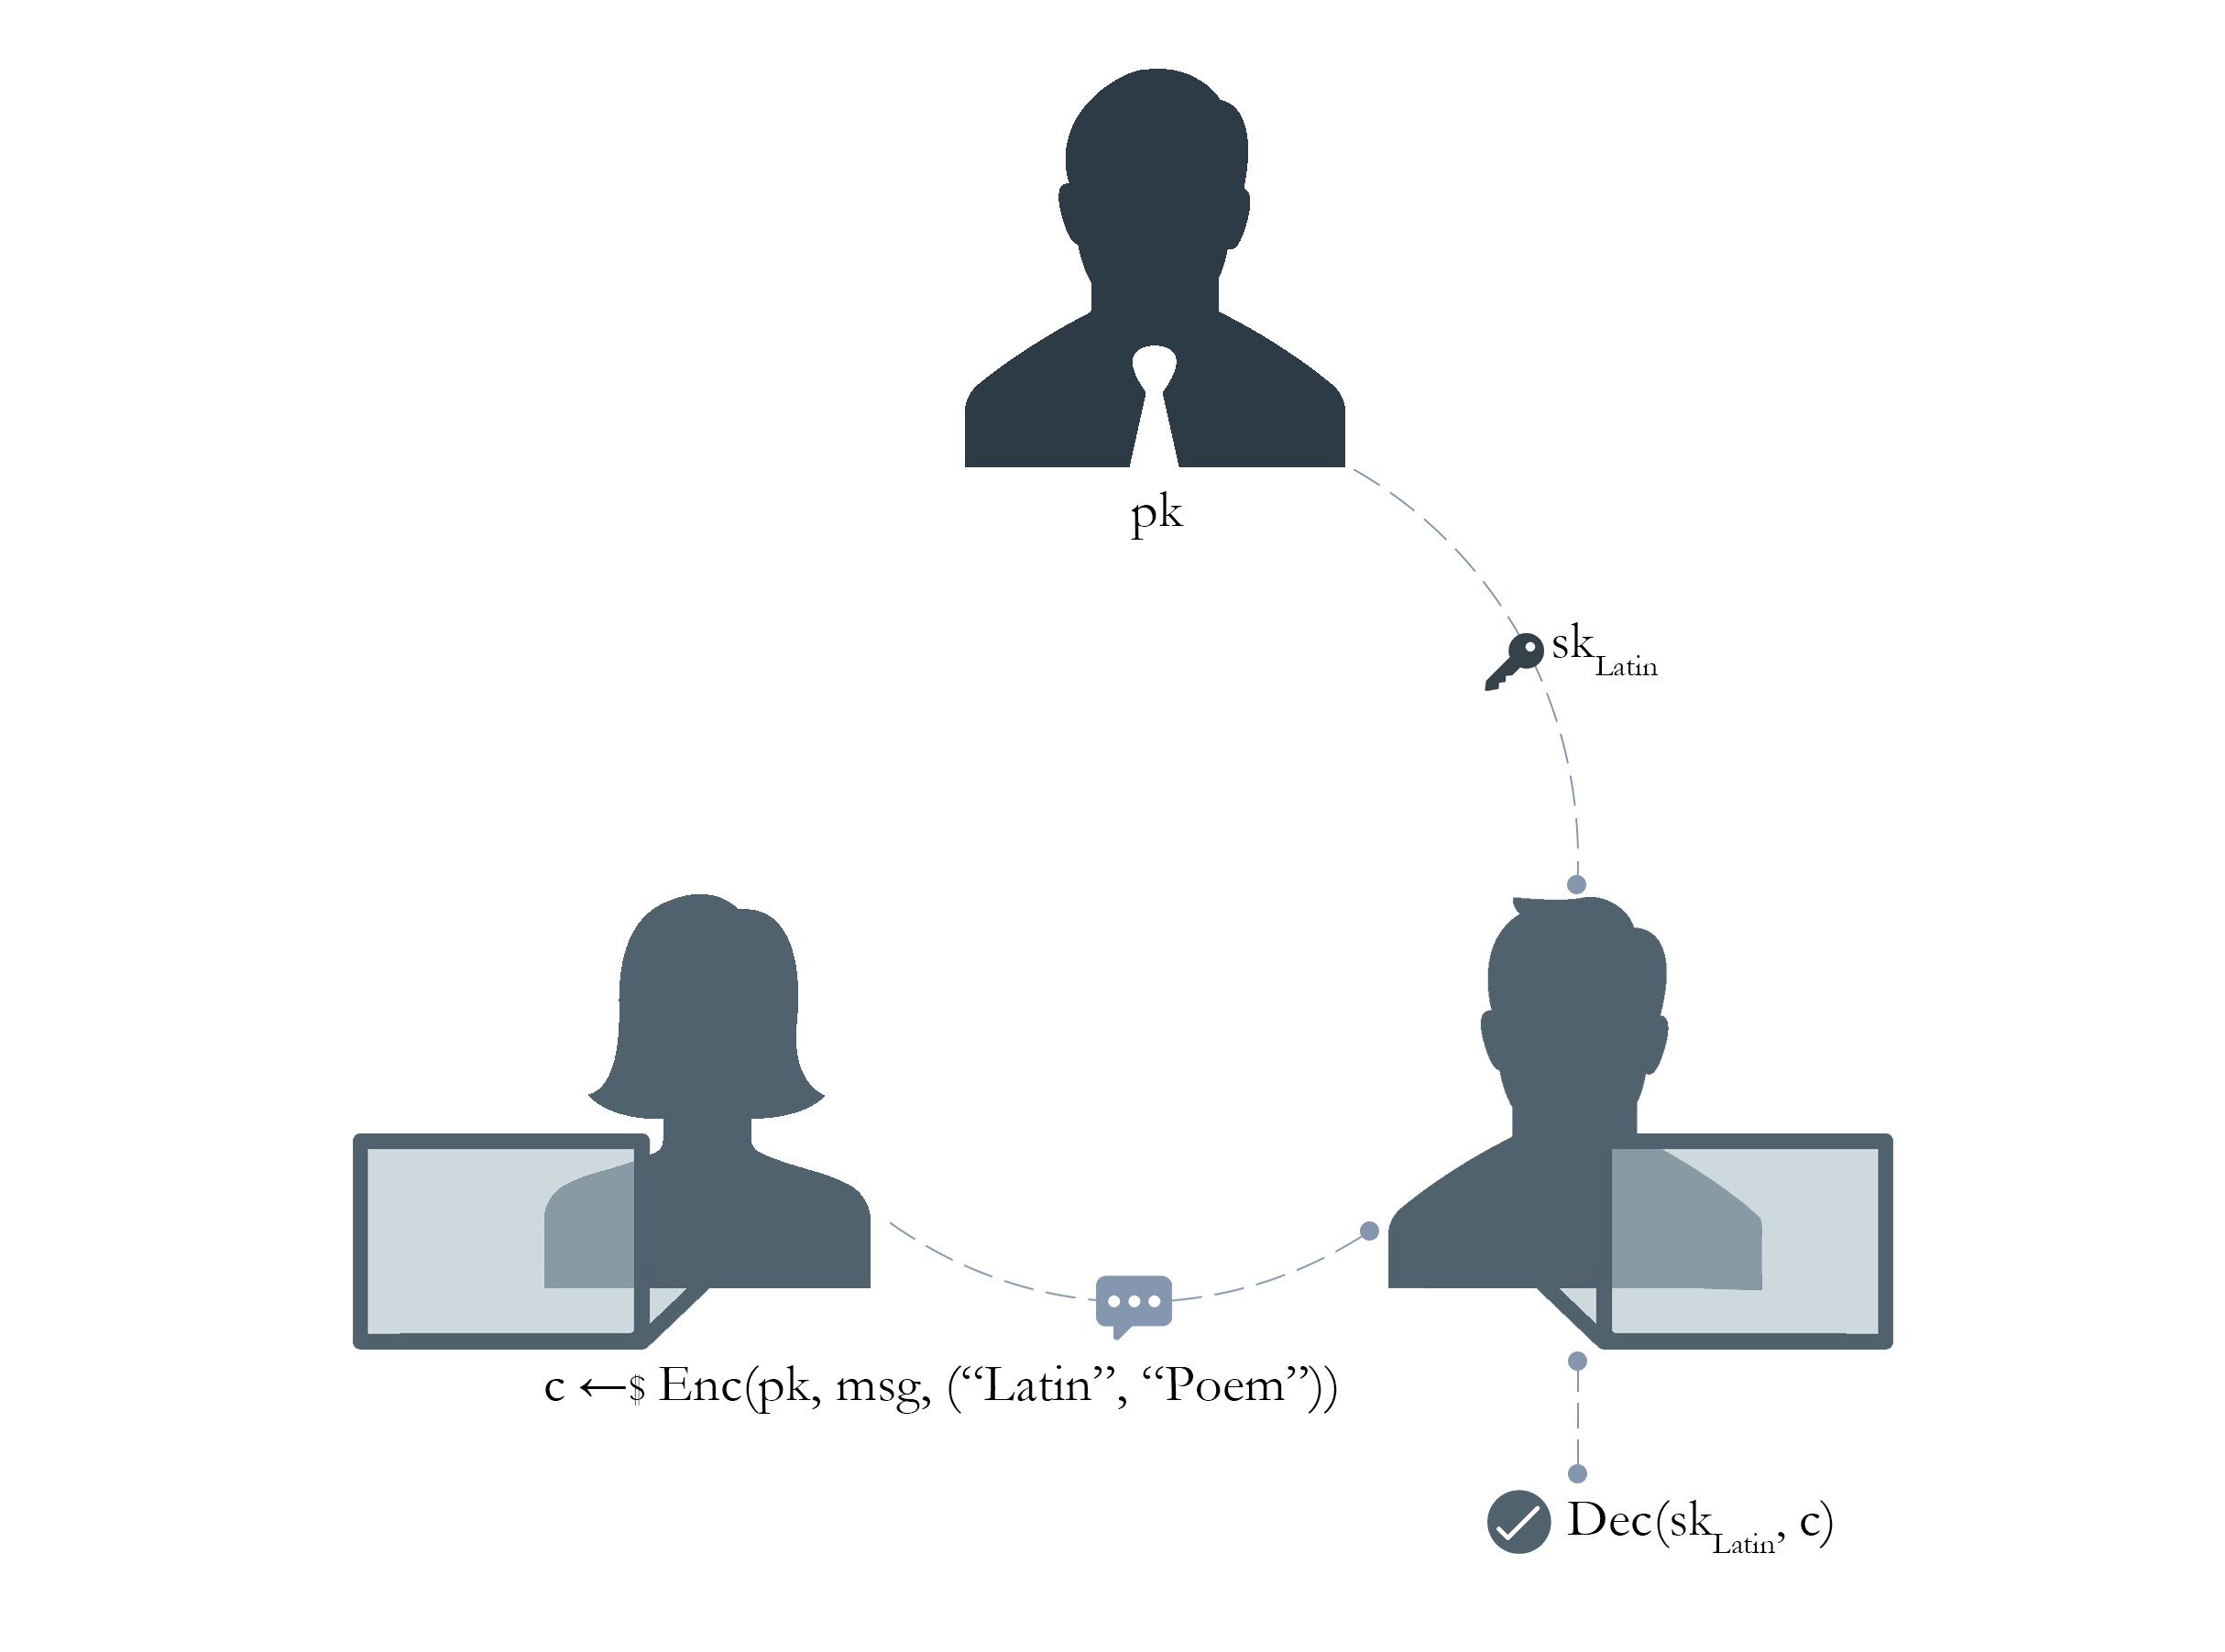
\includegraphics[width=0.8\linewidth]{images/kp_abe.png}
    \caption{KP-ABE example. Alice annotates her message as a Latin poem. Bob is issued some key thanks to which can decrypt any Latin work. In this case, there is a match, i.e. Bob can decrypt the ciphertext.}
    \label{fig:kp_abe_example}
\end{figure}

\paragraph*{Dual-policy ABE}
In ABE, it is clear that only one party can specify a policy, and thus only one user has the possibility to select the source (resp. the destination) of an encrypted message.
Motivated by this limitation, Attrapadung and Imai \cite{Attrapadung} introduced dual-policy ABE.
Here, the sender encrypts a message by choosing both a policy and a set of attributes; the receiver can decrypt the ciphertext using a single decryption key associated with both the receiver's policy and its attributes.
If both policies are satisfied by the respective counterpart, the message is revealed.
